% -----------------------------------------------
% Template for SMC 2012
% adapted from the template for SMC 2011, which was adapted from that of SMC 2010
% -----------------------------------------------

\documentclass{article}
\usepackage{smc2015}
\usepackage{times}
\usepackage{ifpdf}
\usepackage[english]{babel}
\usepackage{cite}

%%%%%%%%%%%%%%%%%%%%%%%% Some useful packages %%%%%%%%%%%%%%%%%%%%%%%%%%%%%%%
%%%%%%%%%%%%%%%%%%%%%%%% See related documentation %%%%%%%%%%%%%%%%%%%%%%%%%%
%\usepackage{amsmath} % popular packages from Am. Math. Soc. Please use the 
%\usepackage{amssymb} % related math environments (split, subequation, cases,
%\usepackage{amsfonts}% multline, etc.)
%\usepackage{bm}      % Bold Math package, defines the command \bf{}
%\usepackage{paralist}% extended list environments
%%subfig.sty is the modern replacement for subfigure.sty. However, subfig.sty 
%%requires and automatically loads caption.sty which overrides class handling 
%%of captions. To prevent this problem, preload caption.sty with caption=false 
%\usepackage[caption=false]{caption}
%\usepackage[font=footnotesize]{subfig}


%user defined variables
\def\papertitle{WEB AUDIO EVALUATION TOOL: A BROWSER-BASED LISTENING TEST ENVIRONMENT} %?
\def\firstauthor{Nicholas Jillings}
\def\secondauthor{Brecht De Man}
\def\thirdauthor{David Moffat}
\def\fourthauthor{Joshua D. Reiss}

% adds the automatic
% Saves a lot of ouptut space in PDF... after conversion with the distiller
% Delete if you cannot get PS fonts working on your system.

% pdf-tex settings: detect automatically if run by latex or pdflatex
\newif\ifpdf
\ifx\pdfoutput\relax
\else
   \ifcase\pdfoutput
      \pdffalse
   \else
      \pdftrue
\fi

\ifpdf % compiling with pdflatex
  \usepackage[pdftex,
    pdftitle={\papertitle},
    pdfauthor={\firstauthor, \secondauthor, \thirdauthor},
    bookmarksnumbered, % use section numbers with bookmarks
    pdfstartview=XYZ % start with zoom=100% instead of full screen; 
                     % especially useful if working with a big screen :-)
   ]{hyperref}
  %\pdfcompresslevel=9

  \usepackage[pdftex]{graphicx}
  % declare the path(s) where your graphic files are and their extensions so 
  %you won't have to specify these with every instance of \includegraphics
  \graphicspath{{./figures/}}
  \DeclareGraphicsExtensions{.pdf,.jpeg,.png}

  \usepackage[figure,table]{hypcap}

\else % compiling with latex
  \usepackage[dvips,
    bookmarksnumbered, % use section numbers with bookmarks
    pdfstartview=XYZ % start with zoom=100% instead of full screen
  ]{hyperref}  % hyperrefs are active in the pdf file after conversion

  \usepackage[dvips]{epsfig,graphicx}
  % declare the path(s) where your graphic files are and their extensions so 
  %you won't have to specify these with every instance of \includegraphics
  \graphicspath{{./figures/}}
  \DeclareGraphicsExtensions{.eps}

  \usepackage[figure,table]{hypcap}
\fi

%setup the hyperref package - make the links black without a surrounding frame
\hypersetup{
    colorlinks,%
    citecolor=black,%
    filecolor=black,%
    linkcolor=black,%
    urlcolor=black
}


% Title.
% ------
\title{\papertitle}

% Authors
% Please note that submissions are NOT anonymous, therefore 
% authors' names have to be VISIBLE in your manuscript. 
%
% Single address
% To use with only one author or several with the same address
% ---------------
%\oneauthor
%   {\firstauthor} {Affiliation1 \\ %
%     {\tt \href{mailto:author1@smcnetwork.org}{author1@smcnetwork.org}}}

%Two addresses
%--------------
% \twoauthors
%   {\firstauthor} {Affiliation1 \\ %
%     {\tt \href{mailto:author1@smcnetwork.org}{author1@smcnetwork.org}}}
%   {\secondauthor} {Affiliation2 \\ %
%     {\tt \href{mailto:author2@smcnetwork.org}{author2@smcnetwork.org}}}



% FIX!!! 
 \fourauthors
   {\firstauthor} {%Affiliation1 \\
     {\tt \href{mailto:b.deman@qmul.ac.uk}{n.g.r.jillings@se14.qmul.ac.uk, }}}
   {\secondauthor} {%Affiliation2\\ %
     {\tt \href{mailto:n.g.r.jillings@se14.qmul.ac.uk}{\{b.deman,}}}
   {\thirdauthor} {%Affiliation3\\ %
     {\tt \href{mailto:d.j.moffat@qmul.ac.uk}{d.j.moffat, }}}
    {\fourthauthor} {%Affiliation4\\ %
     {\tt \href{mailto:joshua.reiss@qmul.ac.uk}{joshua.reiss\}@qmul.ac.uk}}}

% ***************************************** the document starts here ***************
\begin{document}
%
\capstartfalse
\maketitle
\capstarttrue
%
\begin{abstract}
New functionality in HTML5, notably its Web Audio API, allow for increasingly powerful applications in the browser. % is this true?
Perceptual evaluation tests for audio, where the subject assesses certain qualities of different audio fragments through a graphical user interface and/or text boxes, require playback of audio and rapid switching between different files. % what else? 
The advantage of a web application is easy deployment on any platform, without requiring any other application or library, easy storing of results on a server. 
[...]
%Place your abstract at the top left column on the first page.
%Please write about 150-200 words that specifically highlight the purpose of your work,
%its context, and provide a brief synopsis of your results.
%Avoid equations in this part.\\

\end{abstract}
%

\section{Introduction}\label{sec:introduction}
TOTAL PAPER: Minimum 4 pages, 6 preferred, max. 8 (6 for demos/posters)\\ 

NICK: examples of what kind of audio applications HTML5 has made possible, with references to publications (or website)\\

background (types of research where this type of perceptual evaluation of audio is relevant)\\

multiple stimulus perceptual evaluation \cite{bech}\\

prior work: \cite{deman2014b} in MATLAB, much less easy to deploy, and often stops working due to version updates \\ 

goal, what are we trying to do? \\

other background papers (some SMC?)\\

[Previously, due to limited functionality of HTML, ..., it was not possible to design this type of interfaces with such high quality audio... ]


\section{Design considerations}\label{sec:designconsiderations}

We present a browser-based perceptual evaluation tool for audio that ... \\

see \cite{deman2014b}: requirements informed by research on music production (see my work and that of others' in the group), such as randomisation, playback of high quality audio, some degree of flexibility in terms of configuration, ... \\


\section{Implementation}\label{sec:implementation}
%[Nick???]

%section on overall architecture\\

%section with overview of the structure of the input and output files, perhaps with graph or table

The tool runs entirely inside the browser through the new HTML5 Web Audio API. The API is supported by most major web browsers (except Internet Explorer) and allows for constructing a chain of audio processing elements to produce a high quality, real time signal process to manipulate audio streams. The API supports multi-channel processing and has an accurate playback timer for precise scheduled playback control. The Web Audio API is controlled through the browser JavaScript and is therefore highly controllable. The Web Audio API processing is all controlled in a separate thread to the main JavaScript thread, meaning there is no blocking due to real time processing. 

\subsection{Interface}\label{sec:interface} %elsewhere?

[Like \cite{deman2014b}, but others possible]

\begin{figure*}[htbp]
\begin{center}
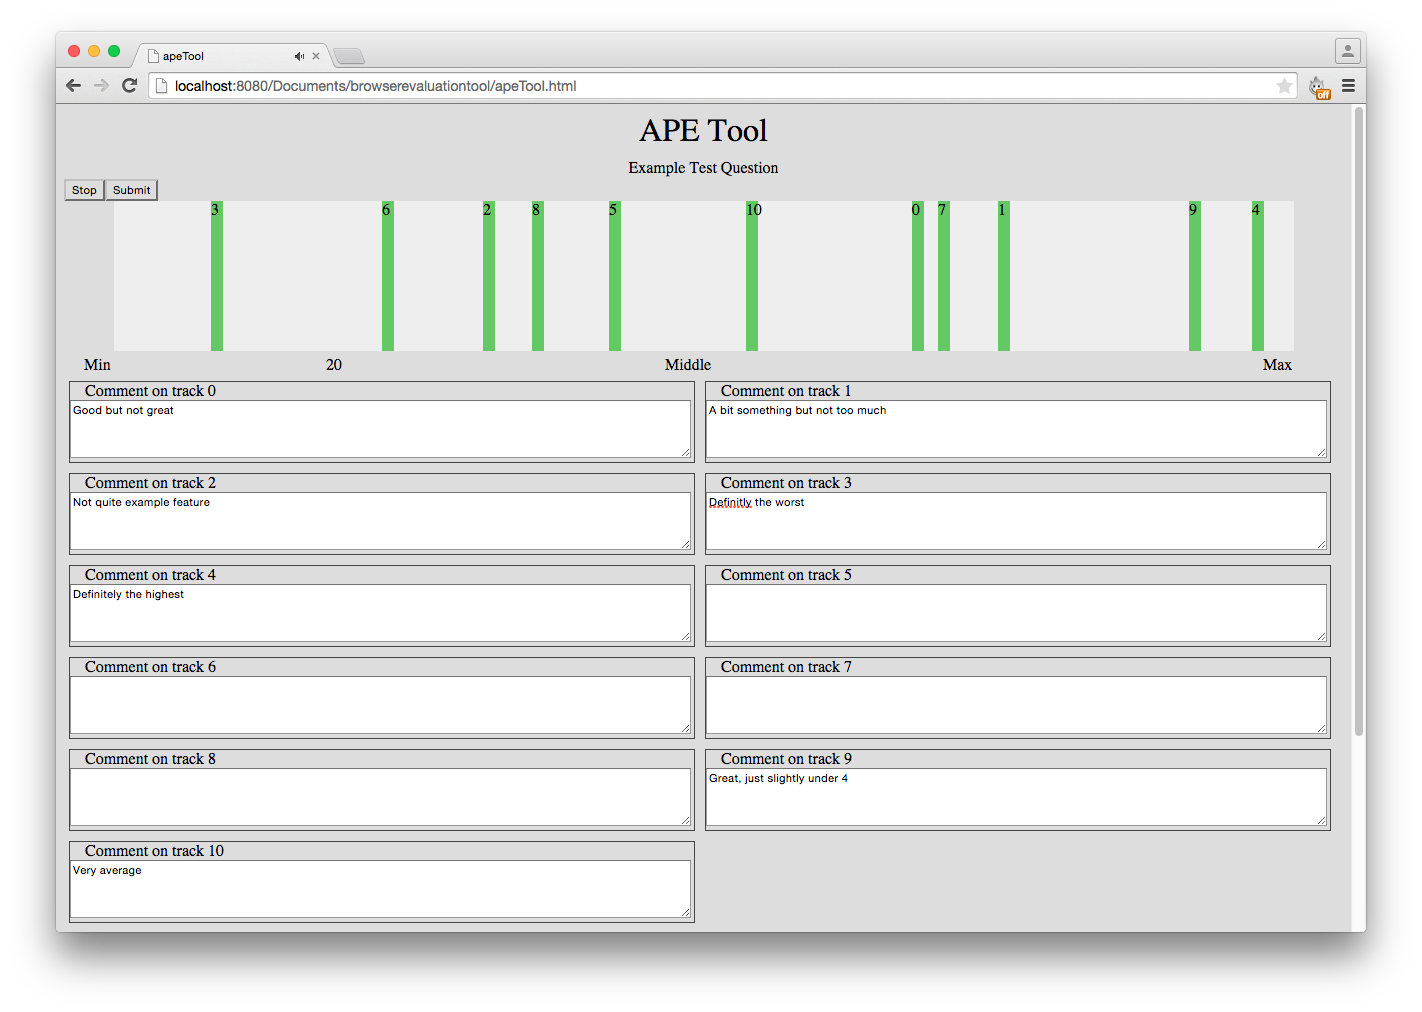
\includegraphics[width=\textwidth]{interface.png}
\caption{Example of interface, with 1 axis and 10 fragments}
\label{fig:interface}
\end{center}
\end{figure*}



\subsection{Architecture}\label{sec:architecture}

The web tool itself is split into several files to operate:
\begin{itemize}
\item \texttt{apeTool.html}: The main index file to load the scripts, this is the file the browser must request to load
\item \texttt{core.js}: Contains functions and objects to manage the audio control, audio objects for testing and loading of files
\item \texttt{ape.js}: Parses setup files to create the interface as instructed, following the same style chain as the MATLAB APE Tool \cite{deman2014b}.
\end{itemize}

The HTML file loads the core.js file with it along with a few other ancillary files (such as the jQuery JavaScript extensions), the browser JavaScript begins to execute the on page instructions, which gives the URL of the test setup XML document (outlined in the next section). The core.js parses this document and executes the function in \texttt{ape.js} to build the web page with the given audio files. The reason for separating these two files is to allow for further interface designs (such as MUSHRA \cite{mushra} or A-B tests \cite{bech}) to be used, which would still require the same underlying core functions outlined in \texttt{core.js}.

The \texttt{ape.js} file has only two main functions: \textit{loadInterface(xmlDoc)} and \textit{interfaceXMLSave()}. The first function is called to build the interface once the setup document has been loaded. This includes creating the slider interface to rate the tracks and creating the comment boxes bellow. The bars in the slider ranking at the top of the page are randomly spaced. It also instructs the audio engine in the \texttt{core.js} to create the audio objects. The audio objects are custom built audio nodes built on the web audio API. They consist of a \textit{bufferSourceNode} (a node which holds a buffer of audio samples for playback) and a \textit{gainNode}. These are then connected to the \textit{audioEngine} (itself a custom web audio node) containing a \textit{gainNode} (where the various Audio Objects connect to) for summation before passing the output to the destination Node, a fixed node created where the browser then passes the audio information to the system sound device.

When an \textit{audioObject} is created, the URL of the audio sample to load is given to it. This is downloaded into the browser asynchronously using the \textit{XMLHttpRequest} object. This allows for downloading of any file into the JavaScript environment for further processing. It is particularly useful for the Web Audio API because it supports downloading of files in their binary form, allowing a perfect copy. Once the asynchronous download is complete, the file is then decoded using the Web Audio API offline decoder. This uses the browser available decoding schemes to decode the audio files into raw float32 arrays, which are in-turn passed to the relevant audioObject bufferSourceNode for playback.

Browsers support various audio file formats and are not consistent in any format. One sure format that all browsers support is the WAV format. Although not a compact, web friendly format, most transport systems are of a high enough bandwidth this should not be a problem. However one problem is that of sample rate. On loading, the browser uses the sample rate assigned by the system sound device. The browser does not have the ability to request a different sound rate. Therefore the default operation when an audio file is loaded with a different sample rate to that of the system is to convert the sample rate. To provide a check for this, the desired sample rate can be supplied with the setup XML and checked against. If the sample rates do not match, a browser alert window is shown asking for the sample rate to be correctly adjusted. This happens before any loading or decoding of audio files. Only once the sample rates match will the system actually fetch any files, keeping down requests for the larger files until they are actually needed.

During playback, the playback nodes loop indefinitely until playback is stopped. The gain nodes in the \textit{audioObject}s enable dynamic muting of nodes. When a bar in the sliding ranking is clicked, the audio engine mutes all \textit{audioObject}s and un-mutes the clicked one. Therefore, if the audio samples are perfectly aligned up and of the same sample length, they will remain perfectly aligned with each other.


\subsection{Setup and Results Formats}\label{sec:setupresultsformats}

Setup and the results both use the common XML document format to outline the various parameters. The setup file contains all the information needed to initialise a test session. Several Nodes can be defined to outline the audio samples to use, questions to be asked and any pre- or post-test questions or instructions. Having one document to modify allows for quick manipulation in a 'human readable' form to create new tests, or adjust current ones, without needing to edit which web files.

The results file is dynamically generated by the interface upon clicking the submit button. There will be checks, depending on the setup file, to ensure that all tracks have been evaluated and their positions in the slider moved. The XML returned contains a node per audioObject and contains its rating in the slider and any comments written in its associated comment box. The rating returned is normalised to be within a integer range of 0 to 100. This normalises the pixel representation of different browser windows. If a window for instance is only 1280 wide, reporting its pixel position is not representative to a display with a width of 1920.

The pre- and post-test options allow for comments or questions to be presented before or after the test. These are automatically generated based upon the given setup XML and allow nearly any form of question and comment to be included in a window on its own. Questions are stored and presented in the response section labelled 'pretest' and 'posttest' along with the question ID and its response. Questions can be made optionally mandatory. Example questions may involve entering mixing experience or listening environment.\\

[LIST OF OPTIONS]\\
% loop, snap to corresponding position, comments, 'general' comment, require same sampling rate, different types of randomisation

[LIST OF THINGS THAT ARE LOGGED] (possibly elsewhere)\\
% time, clicks

The results will also contain information collected by any defined pre/post questions. These are referenced against the setup XML by using the same ID as well as printing in the same question, so readable responses can be obtained. Future development will also evolve to include any session data, such as the browser the tool was used in, how long the test took and any other metrics. Currently the results files are downloaded on the user side of the browser as a .xml file to be manually returned. However the end goal is to allow the XML files to be submitted over the web to a receiving server to store them, allowing for automated collection.

Here is an example of the setup XML and the results XML:
% Should we include an Example of the input and output XML structure?? --> Sure. 

ADD XML STRUCTURE EXAMPLE

\section{Applications}\label{sec:applications} %?
discussion of use of this toolbox (possibly based on a quick mock test using my research data, to be repeated with a large number of participants and more data later)\\

\subsection{Listening Environment Standardisation}

In order to reduce the impact of having a non-standardised listening environment and unobservable participants, a series of pre-test standard questions have been put together to ask every participant. The first part of this is that every participant is asked to carry out the test, wherever possible, with a pair of quality headphones.

% I think the following should be different for every type of test, so I think it looks better to say any type of question (with text box, or radio buttons, or dropdown menu?) is possible to add. 
\begin{itemize}
\item Name (text box)
%\item I am happy for name to be used in an academic publication (check box) % never really necessary, as far as I'm concerned
\item First language (text box)
\item Location: country, city (text box)
\item Playback system (ratio box: headphone or speaker)
\item Make and Model of Playback System (text box)
\item Listening environment (text box)
%\item Please assess how good you believe your hearing to be, where 1 is deaf, 10 is professional critical listener (Dropdown box 1-10 ) % not sure
\end{itemize}


There are also a series of considerations that have been made towards ensuring there is a standardised listening environment, so it is possible to
\begin{itemize}
\item Begin with standardised listening test - to confirm listening experience
\item Perform loudness equalisation on all tracks 
\\** OR THIS SHOULD BE DONE BEFORE THE EXPERIMENT
\item Randomise order of tests
\item Randomise order of tracks in each test
\item Repeat each experiment a number of times 
\\** TO REMOVE THE FAMILIARISATION WITH EXPERIMENT VARIABLE 
\\** TO ENSURE CONSISTENCY OF USER
\item Track all user interactions with system
\end{itemize}


[Regarding randomisation: keep the randomisation 'vector' so you can keep track of what subjects are referring to in comment fields]


\section{Conclusions and future work}\label{sec:conclusions}

In this paper we have presented an approach to creating a browser-based listening test environment that can be used for a variety of types of perceptual evaluation of audio. 
Specifically, we discussed the use of the toolbox in the context of assessment of preference for different production practices, with identical source material. 
The purpose of this paper is to outline the design of this tool, to describe our implementation using basic HTML5 functionality, and to discuss design challenges and limitations of our approach. % or something

% future work
Further work may include the development of other common test designs, such as MUSHRA \cite{mushra}, AB, ABX and method of adjustment tests. 
In addition, [...]. 

%\begin{itemize}
%\item Options for MUSHRA style experiment with vertical slide per track
%\item APE style experiment where all tracks are on a single horizontal axis % isn't that what we're doing now? 
%\item AB test
%\item ABX test
%\item Method of adjustment tests
%\end{itemize}


The source code of this tool can be found on \url{code.soundsoftware.ac.uk/projects/webaudioevaluationtool}. % FIX


%%%%%%%%%%%%%%%%%%%%%%%%%%%%%%%%%%%%%%%%%%%%%%%%%%%%%%%%%%%%%%%%%%%%%%%%%%%%%
%bibliography here
\bibliography{smc2015template}



\end{document}



% RUBBISH

%\subsection{Equations}
%Equations of importance, 
%or to which you refer later,
%should be placed on separated lines and numbered.
%The number should be on the right side, in parentheses.
%\begin{equation}
%E=mc^{2+\delta}.
%\label{eq:Emc2}
%\end{equation}
%Refer to equations like so:
%As (\ref{eq:Emc2}) shows, 
%I do not completely trust Special Relativity.
%
%\subsection{Figures, Tables and Captions}
%\begin{table}[t]
% \begin{center}
% \begin{tabular}{|l|l|}
%  \hline
%  String value & Numeric value \\
%  \hline
%  Hej SMC  & 2015 \\
%  \hline
% \end{tabular}
%\end{center}
% \caption{Table captions should be placed below the table, exactly like this,
% but using words different from these.}
% \label{tab:example}
%\end{table}

%\begin{figure}[t]
%\figbox{
%\subfloat[][]{\includegraphics[width=60mm]{figure}\label{fig:subfigex_a}}\\
%\subfloat[][]{\includegraphics[width=80mm]{figure}\label{fig:subfigex_b}}
%}
%\caption{Here's an example using the subfig package.\label{fig:subfigex} }
%\end{figure}





%\begin{acknowledgments}
%You may acknowledge people, projects, 
%funding agencies, etc. 
%which can be included after the second-level heading
%``Acknowledgments'' (with no numbering).
%\end{acknowledgments} 

